\documentclass[12pt]{article}
\usepackage[utf8]{inputenc}
\usepackage[T1]{fontenc}
\usepackage{amsmath}
\usepackage{geometry}
\usepackage{graphicx}
\usepackage{makeidx}
\geometry{margin=2.5cm}
\usepackage{fancyhdr}

\begin{document}
	
	\thispagestyle{empty}
	
	\begin{center}
		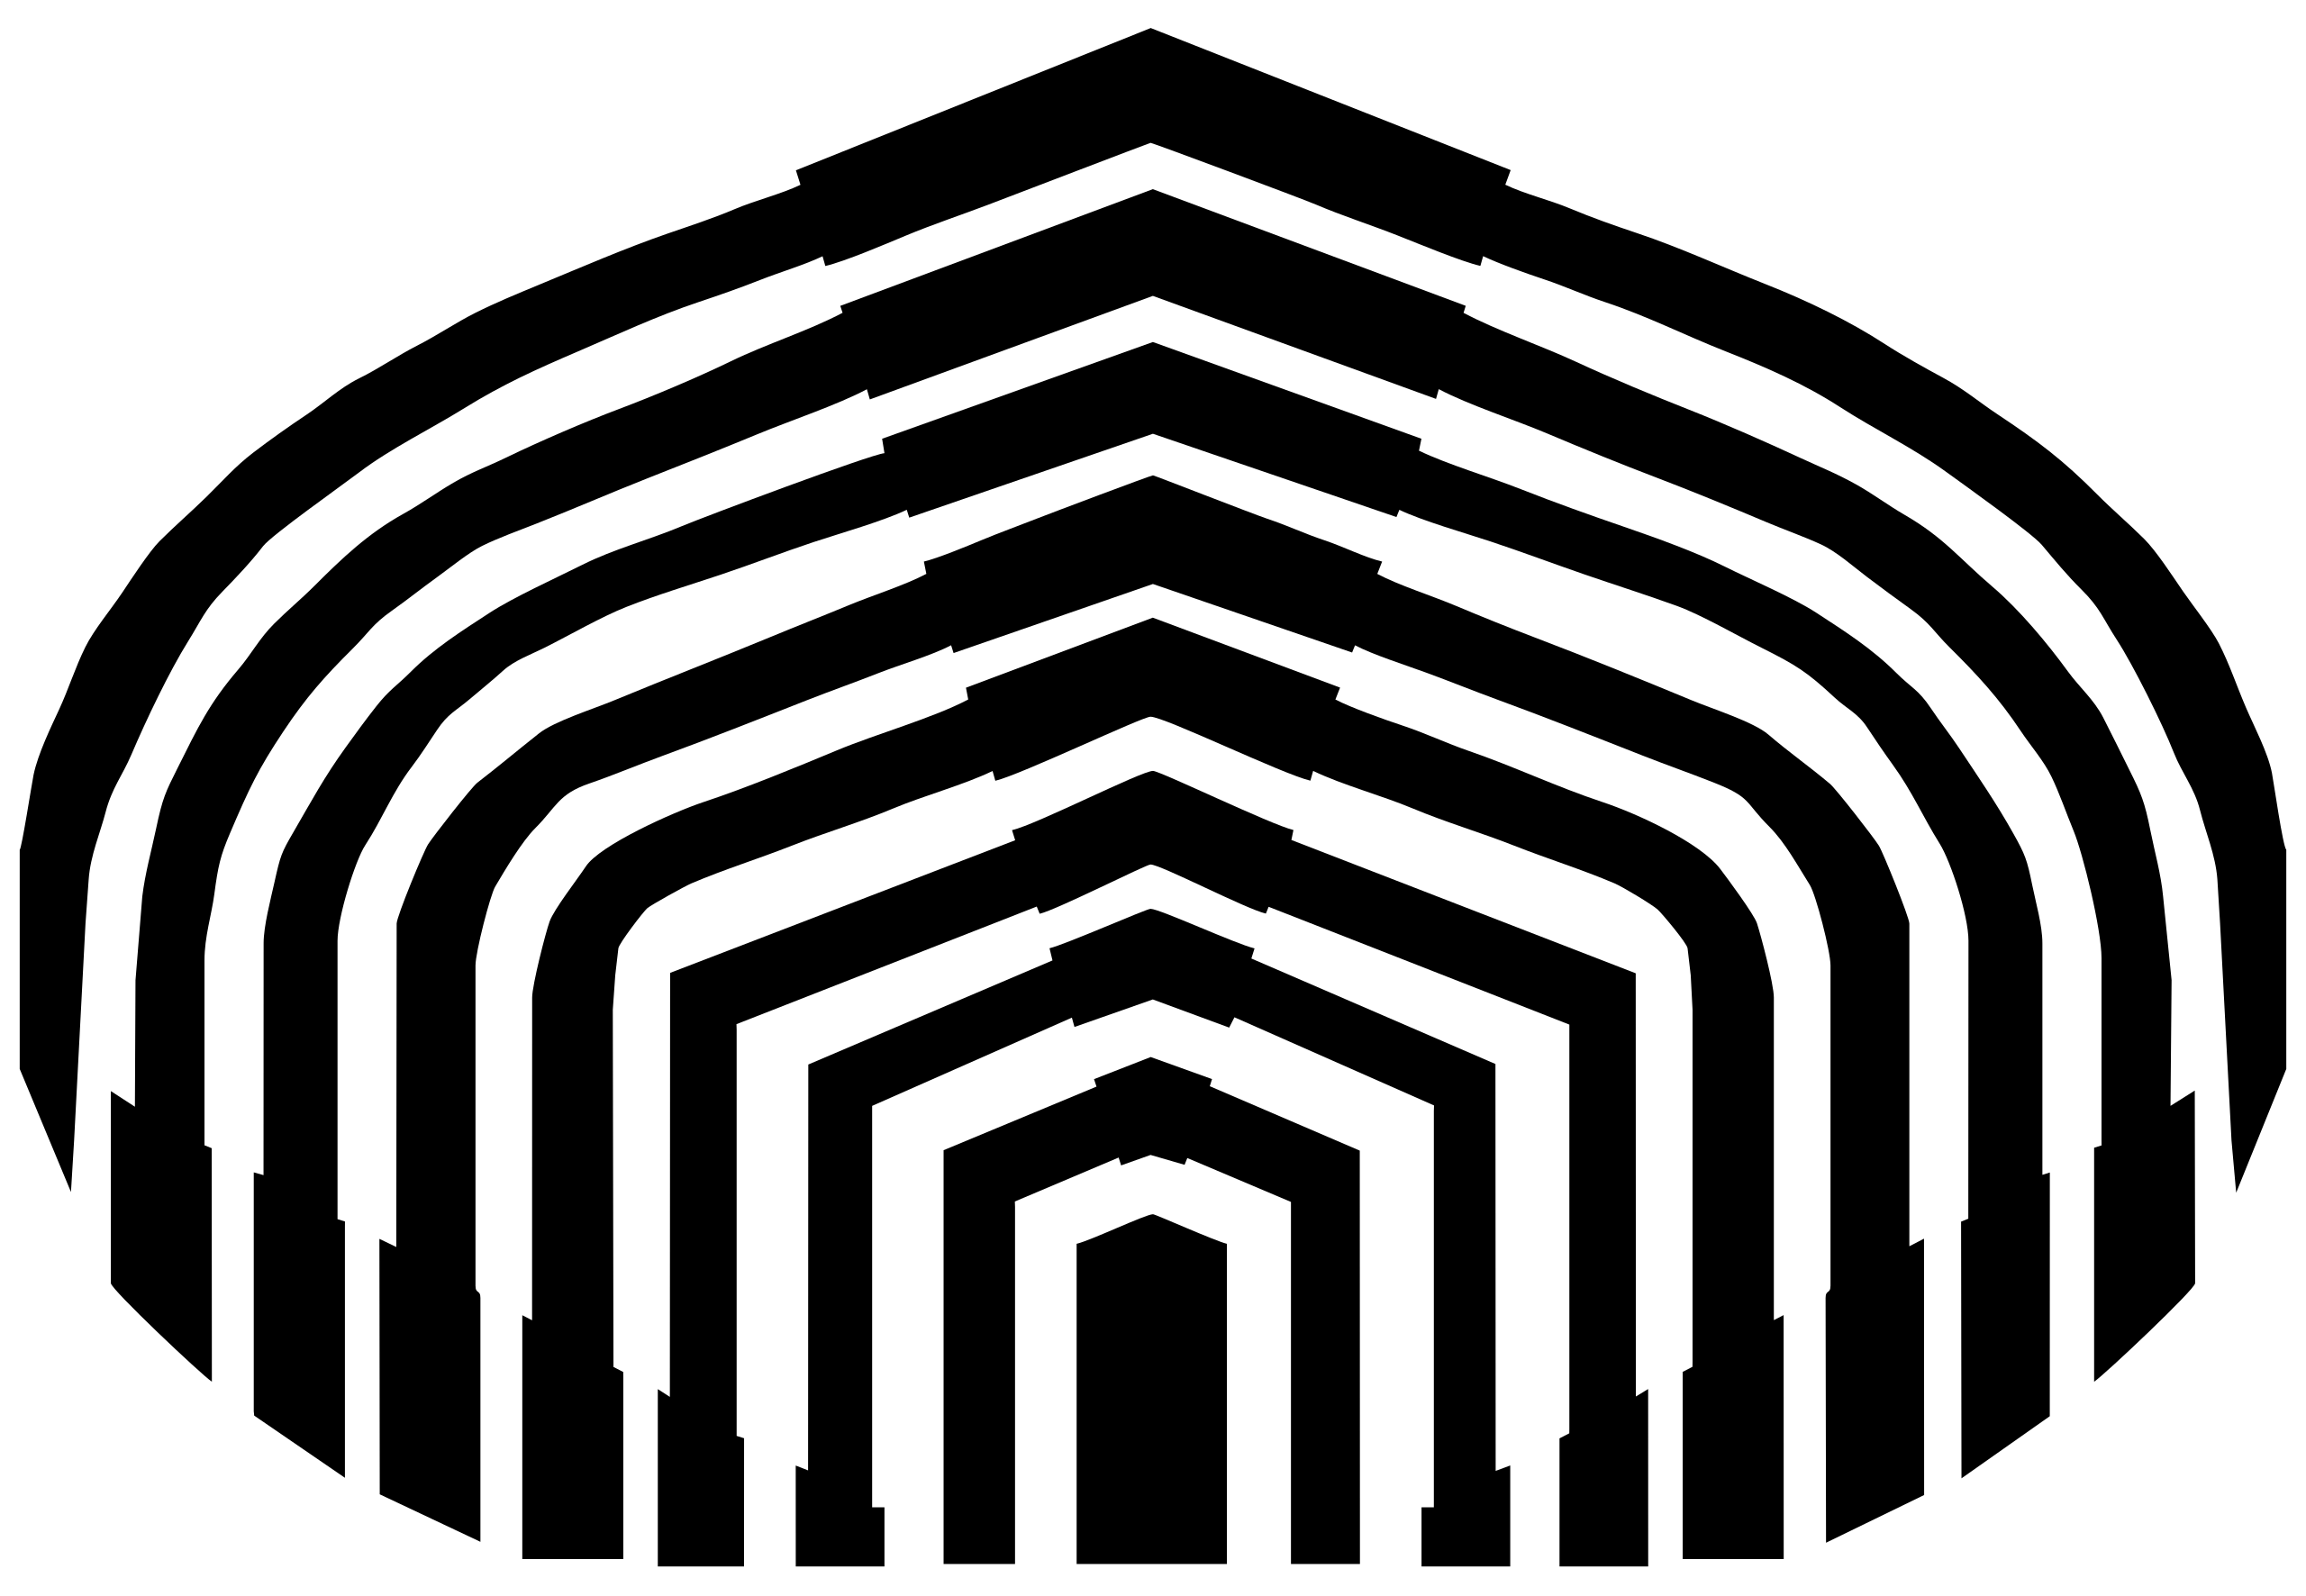
\includegraphics[width=3.1cm,height=2cm]{logo}\\
		UNIVERSIDAD SIMÓN BOLÍVAR\\
		DEPARTAMENTO DE ELECTRÓNICA Y CIRCUITOS\\
		EC1281 - LABORATORIO DE MEDICIONES ELÉCTRICAS\\
		SECCIÓN 1 - GRUPO 1\\
		
		\vspace{7cm}
		\textbf{\Large INFORME - PRÁCTICA \#4}\\
		EL OSCILOSCOPIO\\
	\end{center}
	
	\begin{flushleft}
		\vspace{9cm}
		\hfill Integrantes:\\
		\hfill {\large Luis Becerra - 1910557}\\
		\hfill {\large Lorena Rojas - 1910469}\\
	\end{flushleft}
	
	\newpage
	
	\pagenumbering{Roman}
        \setcounter{page}{2}
	
	\begin{center}
		\textbf{\large RESUMEN}\\
	\end{center}
	
	Inserte resumen
	
	\newpage
	
	\begin{center}
		\textbf{\large ÍNDICE}\\
	\end{center}
	
	\noindent \textbf{RESUMEN} \hfill \textbf{II}\\
	\noindent \textbf{ÍNDICE} \hfill \textbf{III}\\
	\noindent \textbf{MARCO TEÓRICO} \hfill \textbf{1}\\
	\noindent \textbf{METEDOLOGÍA} \hfill \textbf{4}\\
	\noindent \textbf{RESULTADOS} \hfill \textbf{5}\\
	\noindent \textbf{ANÁLISIS DE RESULTADOS} \hfill \textbf{13}\\
	\noindent \textbf{CONCLUSIONES} \hfill \textbf{14}\\
	\noindent \textbf{BIBLIOGRAFÍA} \hfill \textbf{15}\\
	\noindent \textbf{ANEXOS} \hfill \textbf{16}\\
	
	\newpage
	
	\pagenumbering{arabic}
	
	\begin{center}
		\textbf{\large MARCO TEÓRICO}\\
	\end{center}
	
	\textbf{1. }\\
	
	Inserte inciso 1
	
	\begin{itemize}
		\item \textbf{Sub-elemento 1 del inciso } inserte lo que corresponda
		
	\end{itemize}

	\newpage
	
	\begin{center}
		\textbf{\large METODOLOGÍA}\\
	\end{center}
	
	\renewcommand{\theenumi}{\alph{enumi}} %Letras minúsculas 
	
	\begin{enumerate}
		
		\item Determinación experimental del equivalente Thevenin:\\
		
		Tal y como se estudió en EC1251, el teorema de Thevenin es una simplificación que podemos aplicar para circuitos con elementos lineales, donde se reduce el circuito a un voltaje de Thevenin y una resistencia de Thevenin entre dos puntos $A$ y $B$. El equivalente de Thevenin de un circuito permite facilitar la operación del mismo respecto a un par de nodos de interés, haciendo mucho más simples los cálculos y manipulación del mismo. El circuito al cual se le determinó el equivalente de Thevenin fue:
		
		\begin{center}
			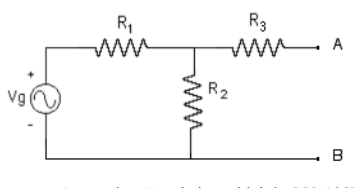
\includegraphics[width=16cm,height=8cm]{Img/circ_1}
		\end{center}
		
		Los valores nominales utilizados para este circuito fueron $V_g = 5V$, $f = 100Hz$, $R_1 = R_2 = 2k\Omega$ y $R_3 = 1k\Omega$.\\
		
		A partir de esos valores y esa configuración de circuito se procedió a realizar algunas medidas para calcular el equivalente de Thevenin. Se midió el voltaje de Thevenin mediante el osciloscopio y un voltímetro, también se midió la corriente de Norton con un amperímetro y con el osciloscopio usando una resistencia de $51,3\Omega$. Con el osciloscopio se obtuvieron los valores pico. A partir de eo datos se desarrolló se obtuvo el valor de Thevenin para las resistencias.\\
		
		\item Teorema de Máxima transferencia de Potencia:\\
		
		El teorema de máxima transferencia de potencia establece que, dada una fuente, con una resistencia de fuente fijada, la resistencia de carga que maximiza la transferencia de potencia es aquella con un valor óhmico igual a la resistencia de fuente.\\
		
		De allí se obtiene la idea de cómo variar la resistencia para obtener la máxima potencia, en los experimentos se realizan dos configuraciones, la primera variando la resistencia de Thevenin y la segunda variando la resistencia $R_L$.
		
		\begin{center}
			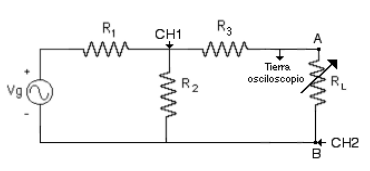
\includegraphics[width=16cm,height=8cm]{Img/circ_2}
		\end{center}
	
		\begin{center}
			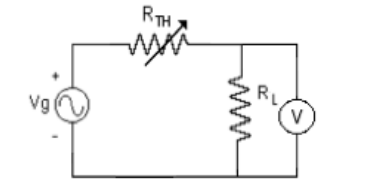
\includegraphics[width=16cm,height=8cm]{Img/circ_3}
		\end{center}
	
		A partir de allí se usaron las mismas resistencias y $V_g$ que antes, en el caso en el que se varía la resistencia de Thevenin se usó una resistencia de $2k\Omega$.
		
		\item Impedancias en un circuito:\\
		
		Para este experimento se usó un circuito al cual se le tomaron mediciones en distintos puntos, los cuales fueron:\\
		
		\begin{center}
			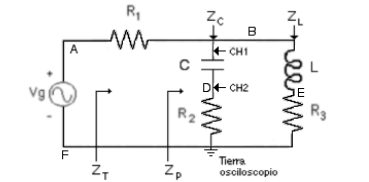
\includegraphics[width=16cm,height=8cm]{Img/circ_4}
		\end{center}
	
		\begin{center}
			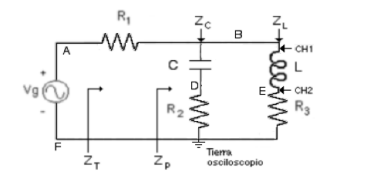
\includegraphics[width=16cm,height=8cm]{Img/circ_5}
		\end{center}
		
		\begin{center}
			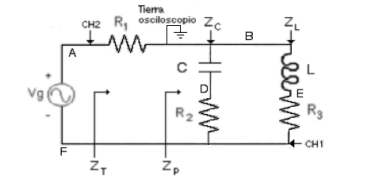
\includegraphics[width=16cm,height=8cm]{Img/circ_6}
		\end{center}
	
		Y a partir de allí se determinaron las impedancias y el defase partiendo de tres resistencias cuyo valor nominal era $1k\Omega$, un condensador de $100nF$, un inductor de $100mH$ y una fuente de $10V$ pico a $1kHz$. Luego siguiendo leyes circuitales se determinó la impedancia.
		
		\item Operación de un medidor de verdadero valor rms y un vatímetro digital:\\
		
		Para este experimento se usó un variac, un dimmer, un bombillo y los distintos aparatos de medición. Lo que se hizo fue que primero se variaba el voltaje con el variac para modificar el la potencia disipada en el bombillo y tomar las medidas en los distintos instrumentos, luego, se realizó el mismo proceso con el dimmer, un aparato para regular la potencia disipada sin disminuir el voltaje.
		
		
	\end{enumerate}
	
	\newpage
	
	\begin{center}
		\textbf{\large RESULTADOS}\\
	\end{center}
	
	Inserte resultados
	
	\newpage
	
	\begin{center}
		\textbf{\large ANÁLISIS DE RESULTADOS}\\
	\end{center}
	
	\renewcommand{\theenumi}{\alph{enumi}} %Letras minúsculas 
	
	\begin{enumerate}
		
		\item Mediciones del valor pico y el valor
		rms para las tres señales periódicas a diferentes frecuencias:
		
	\end{enumerate}
	
	\newpage
	
	\begin{center}
		\textbf{\large CONCLUSIONES}\\
	\end{center}
	
	Inserte conclusiones
	
	\newpage
	
	\begin{center}
		\textbf{\large BIBLIOGRAFÍA}\\
	\end{center}
	
	Inserte bibliografía
	
	\newpage
	
	\begin{center}
		\textbf{\large ANEXOS}\\
	\end{center}
	
	Inserte anexos
	
\end{document}
